
\chapter{Kính hiển vi}
\section{Lý thuyết trọng tâm}

\subsection{Công dụng và cấu tạo của kính hiển vi}
Kính hiển vi là một dụng cụ quang học bổ trợ cho mắt dùng để quan sát
những vật rất nhỏ bằng cách tạo ảnh có góc trông lớn.

Kính hiển vi có hai bộ phận chính:
\begin{itemize}
	\item \textbf{Vật kính} $L_1$ là một thấu kính hội tụ (thực ra là một hệ thấu kính tác dụng như thấu kính hội tụ) có tiêu cự rất nhỏ (cỡ milimét).
	\item \textbf{Thị kính} $L_2$ là một kính lúp dùng để quan sát ảnh của vật tạo bởi vật kính.
	\end{itemize}
\begin{center}
	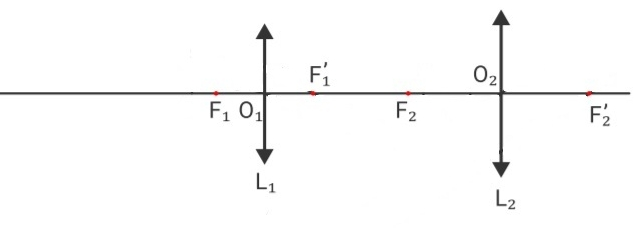
\includegraphics[scale=0.4]{../figs/VN11-PH-42-L-030-1-h52.jpg}
\end{center}
Hai bộ phận chính này được gắn ở hai đầu của một ống trụ sao cho trục chính của chúng trùng nhau và khoảng cách giữa chúng $\text{O}_1\text{O}_2=l$ không đổi.

Người ta gọi $\text{F'}_1\text{F}_2=\delta$ là \textit{độ dài quang học} của kính.

\subsection{Sự tạo ảnh bởi kính hiển vi}
\begin{center}
	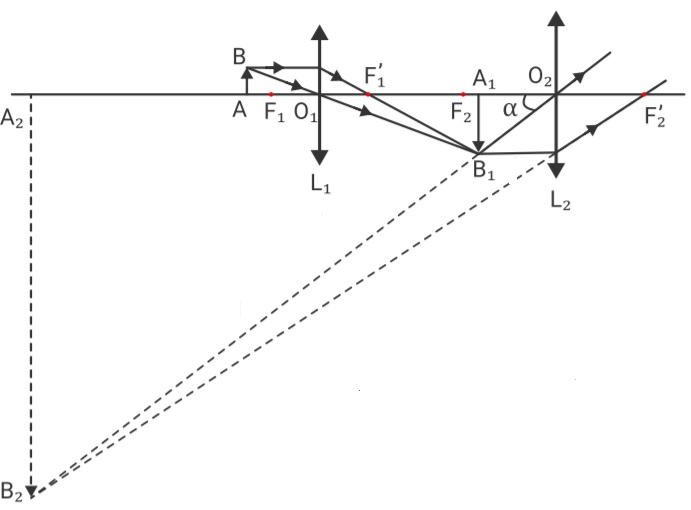
\includegraphics[scale=0.7]{../figs/VN11-PH-42-L-030-1-h51.jpg}
\end{center}
\begin{itemize}
	\item Vật kính có tác dụng tạo ảnh thật $\text{A}_1\text{B}_1$ lớn hơn vật AB và ở trong khoảng
	$\text{O}_2\text{F}_2$ từ quang tâm đến tiêu diện vật của thị kính.
	\item Thị kính tạo ảnh ảo sau cùng $\text{A}_2\text{B}_2$ lớn hơn vật nhiều lần và ngược chiều
	so với vật AB.
\end{itemize}


\subsection{Số bội giác của kính lúp khi ngắm chừng vô cực}
\begin{equation}
G_\infty=|k_1|\cdot G_2,
\end{equation}
trong đó,
\begin{itemize}
	\item $G_\infty$ là số bội giác của kính hiển vi khi ngắm chừng vô cực,
	\item $|k_1|$ là độ lớn số phóng đại ảnh bởi vật kính,
	\item $G_2$ là số bội giác của thị kính khi ngắm chừng ở vô cực. 
\end{itemize}

Công thức trên có thể biến đổi và viết dưới một dạng khác:
\begin{equation}
G_\infty=\dfrac{\delta \cdot \text{Đ}}{f_1\cdot f_2},
\end{equation}
trong đó,
\begin{itemize}
	\item $\delta$ là độ dài quang học của kính,
	\item $\text{Đ}$ là khoảng cực cận của mắt,
	\item $f_1$ là tiêu cự của vật kính,
	\item $f_2$ là tiêu cự của thị kính.
\end{itemize}


\section{Bài tập }
\begin{dang}{Ngắm chừng ở vô cực}
\end{dang}
\textbf{Phương pháp giải}

Sử dụng công thức tính số bội giác khi ngắm chừng vô cực:
\begin{equation*}
G_\infty=|k_1|\cdot G_2,
\end{equation*}
hoặc 
\begin{equation*}
G_\infty=\dfrac{\delta \cdot \text{Đ}}{f_1\cdot f_2},
\end{equation*}
tùy vào dữ kiện mà đề bài cung cấp. Khoảng cực cận Đ của mắt thường là $25\ \text{cm}$.

\vspace*{1em}
\viduii{2}{
Một người mắt tốt có khoảng nhìn rõ từ 25 cm đến vô cực, quan sát một vật nhỏ qua kính hiển vi có vật kính $\text{O}_1\ (f_1=1\ \text{cm})$ và thị kính $\text{O}_2\ (f_2=5\ \text{cm})$.  Khoảng cách $\text{O}_1\text{O}_2=20\ \text{cm}$ Độ bội giác của kính hiển vi trong trường hợp ngắm chừng ở vô cực là
\begin{mcq}(4)
	\item 67.
	\item 70.
	\item 100.
	\item 120.
\end{mcq}}{
\begin{center}
	\textbf{Hướng dẫn giải:}
\end{center}

{ Đề bài cho khoảng cực cận $\text{Đ}= 25\ \text{cm}$, $f_1=1\ \text{cm}, \ f_2=5\ \text{cm}$.

Độ dài quang học $\delta=\text{F'}_1\text{F}_2=\text{O}_1\text{O}_2-f_1-f_2=14 \ \text{cm}$.
 
$ G_\infty=\dfrac{\delta \cdot \text{Đ}}{f_1\cdot f_2}=70$.

\textbf{	Đáp án: B.}
}
}
\viduii{2}{
Số phóng đại của vật kính của kính hiển vi bằng 30. Biết tiêu cự của thị kính là 2 cm, khoảng cực cận của người quan sát là 25 cm. Số bội giác của kính hiển vi đó khi ngắm chừng ở vô cực là
\begin{mcq}(4)
	\item 350.
	\item 375.
	\item 400.
	\item 425.
\end{mcq}}{
\begin{center}
	\textbf{Hướng dẫn giải:}
\end{center}

{ Đề bài cho khoảng cực cận $\text{Đ}= 25\ \text{cm}$, $k_1=30, \ f_2=2\ \text{cm}$.
	
	$ G_\infty=|k_1|\cdot G_2=|k_1|\cdot \dfrac{\text{Đ}}{f_2}=375$.
	
\textbf{	Đáp án: B.}
}
}